\section{Results in the Nominal Basis}\label{sec:eft_nominal_basis_results}
Maximum likelihood fits (\cref{sec:stats_mle}) are performed to extract individual constraints on the 43 Wilson coefficients when fixing the other Wilson coefficients to their SM values of zero. The observed best-fit values, and 68\% and 95\% CL intervals are shown in \cref{fig:smeft_results_nominal_observed} when using the SMEFT parameterization up to linear order only, or up to quadratic order (linear-plus-quadratic). Also shown are the 95\% CL lower limits on the probed energy scale, $\Lambda$, when assuming $c_i=1$. 

In general, the results show good agreement with the SM, with the $C_{HG}$ and $C_{HB}$ coefficients showing the tightest constraints corresponding to probed energy scales of up to 15\TeV. The most discrepant result is that for $C_{Hq}^{(3)}$, which has a p-value with respect to the SM hypothesis of 0.01, regardless of whether the linear or up to quadratic parameterization is used. This discrepancy is expected because this coefficient has its highest impact in the high \ptV \WH and \ZH leptonic bins, which saw the largest disagreements with the SM in the STXS measurements (\cref{fig:stxs_stage1p2_results}).

The largest differences between the results when using the linear and linear-plus-quadratic parameterizations is seen for poorly constrained coefficients, where in some more extreme cases, the coefficients cannot be constrained with the linear contributions alone. This trend is expected because when $C \ll 1$, the quadratic terms are suppressed but as $C$ becomes larger, there is less suppression. These differences are important to remember when considering the results in the rotated basis which is restricted to use the linear parameterization.

\begin{figure}
  \centering
  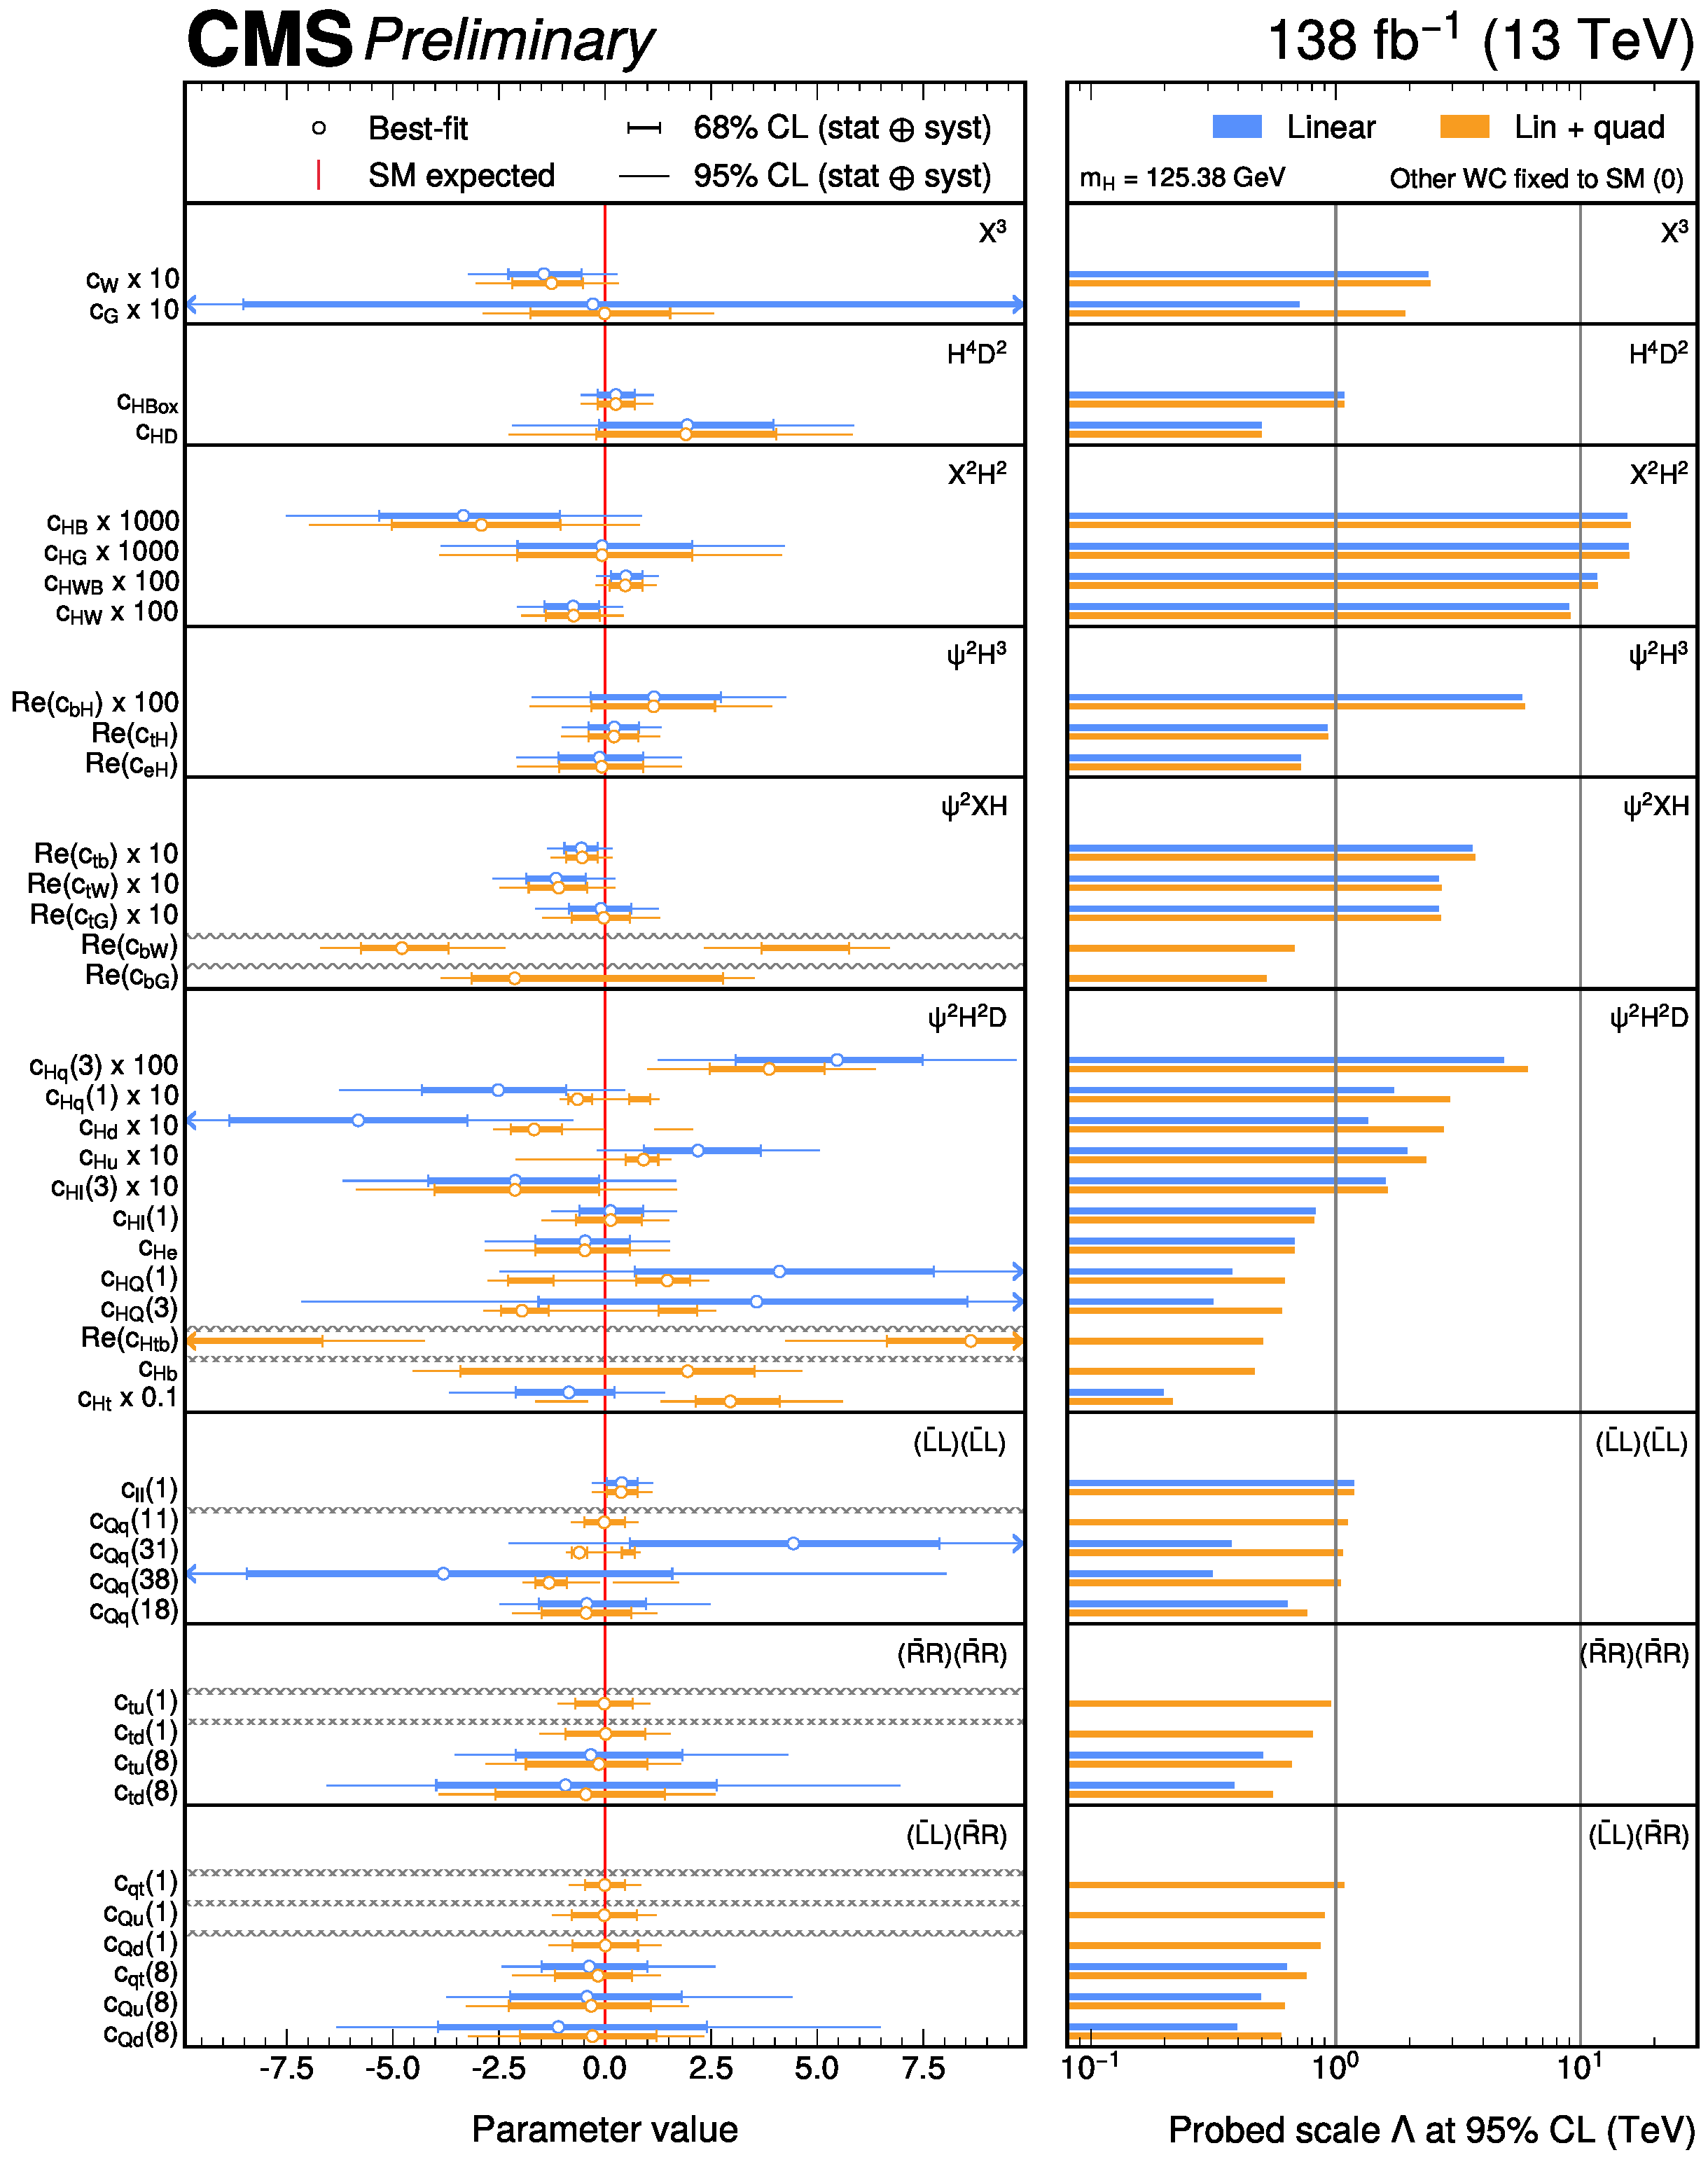
\includegraphics[width=\textwidth]{Figures/EFT/HIG-21-018-Figure_017.pdf}
  \caption[Individual Constraints on the SMEFT Wilson Coefficients]{Observed constraints on the individual Wilson coefficients when setting the values of the other coefficients to zero. The left panel shows the best-fit values, the SM expectation ($C=0$), and the 68\% and 95\% CL intervals. The results from the linear and linear-plus-quadratic parameterizations are shown in blue and orange respectively. For the linear parameterization, some coefficients are not constrained, which is indicted by a hatched line. When a confidence interval extends beyond the range of the plot, it is indicated by an arrow. The right panel shows the 95\% CL lower limits on the probed energy scale, $\Lambda$, when assuming $c_i=1$.}\label{fig:smeft_results_nominal_observed}
\end{figure}